\section{Assumptions and Dependencies}
\begin{itemize}
	\item Operating System: Linux/Windows
	\item Processor Speed: 512KHz or more
	\item RAM: Minimum 2GB
	\item Library: Mapnik
	\item Modules: Mod\_tile
	\item Compiler: CartoCSS
	\item Stylesheet: OSMBright
	\item Programming Language: C++, Python
\end{itemize}

\subsection{Dependency Graph}
A Dependency Graph is a graphical representation of the which module is dependent on which other modules. A Dependency Graph is often used as a preliminary step to creating an overview of the system. Dependency Graph also gives overview of how good is the design of the system.
FreeCAD being were huge software it would be difficult to make the dependency graph of whole software. So, here is  Dependency Graph of openstreetmap-carto is as following:
\begin{enumerate}
\item \textbf{Caller graph of osmium index object:} Figure \ref{fig:comment1} shows the modules that use Key-value containers with unique integer values for a key.
\item \textbf{Caller graph of expiration of the tiles in osm2pgsql:} Figure \ref{fig:comment} shows the modules that expire the tile in osm2pgsql. If bounding box too big - just expire tiles on the line
\item \textbf{Caller graph to generate\_road\_colours:} Figure \ref{fig:dependency} show the modules that generate the road colurs based on primary, secondary roads.

\item \textbf{Caller graph of tag tranform in postgresql:} Figure \ref{fig:dependencyy} show the modules that uses tags tranform with transform lua filters.
\end{enumerate}

\begin{figure}
	\centering
	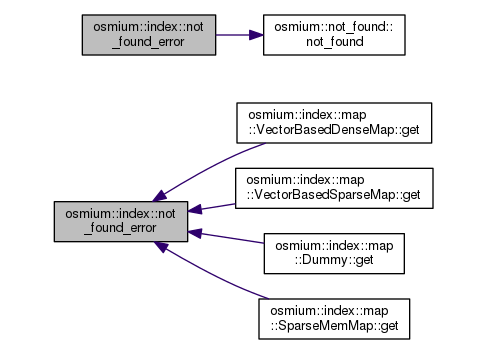
\includegraphics[scale=.8]{input/images/dep_osmium_index.png}
	\caption{Dependency graph of osmium index object}
	\label{fig:comment1}
\end{figure}

\begin{figure}
\centering
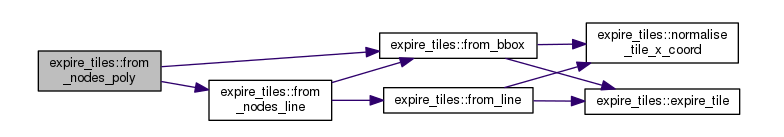
\includegraphics[width=1\linewidth]{input/images/dep_expire_tiles.png}
\caption{Caller graph of expiration of the tiles in osm2pgsql}
\label{fig:comment}
\end{figure}
\begin{figure}
\centering
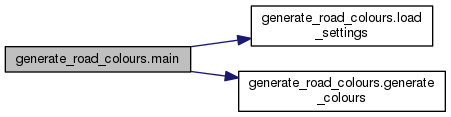
\includegraphics[scale=0.8]{input/images/dep_road.png}
\caption{Caller graph to generate\_road\_colours}
\label{fig:dependency}
\end{figure}


\begin{figure}
\centering
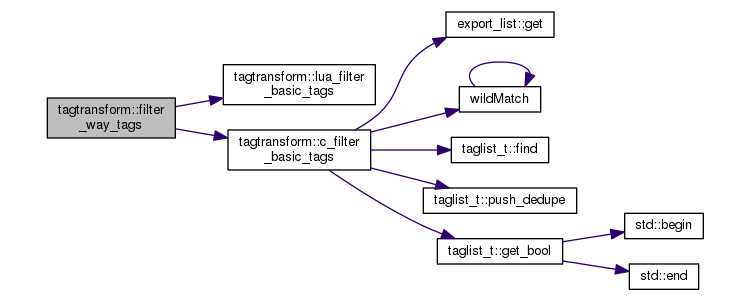
\includegraphics[scale=0.6]{input/images/dep_tagtransform.png}
\caption{Caller graph of tag tranform in postgresql}
\label{fig:dependencyy}
\end{figure}


\subsection{Class Diagrams}
Class Diagrams describe the static structure of the system. Following classes diagram represent the relationship between different classes in :
\begin{enumerate}
	\item Figure \ref{fig:collaborative1} shows the class diagram of the road colours class which is the base class of which is the base class of lch, rgb, CIE color space.

\iffalse

	\item Figure \ref{fig:collaborative} shows the class diagram of the tagstranform which is the main class of database\_options, lua filter tags, bbox, hstore\_columns, slim, cache.
	
	\item Figure \ref{fig:classAnnotation__coll__graph}  shows the class diagram of the osmdata which is the main class of node\_add, way\_add, relation\_add, relation\_modify, node\_delete, way\_delete, relation\_delete.

\fi

	\item Figure \ref{fig:classAnnotation__coll__graphh}  shows the inheritance diagram of reprojecion which has target\_latlon, target\_to\_tile, reproject, create\_projection.
\end{enumerate}

\begin{figure}
    \centering
    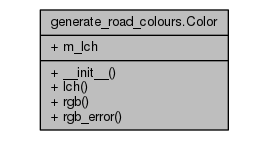
\includegraphics[scale=.85]{input/images/class_road.png}
    \caption{Class Diagram for generating road colours}
    \label{fig:collaborative1}
\end{figure}

\iffalse

\begin{figure}
    \centering
    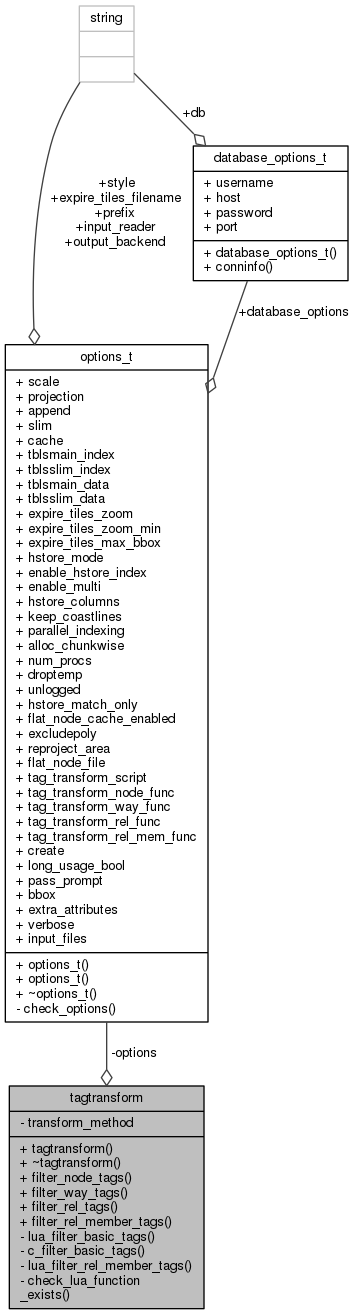
\includegraphics[scale=.5]{input/images/class_tagtransform.png}
    \caption{Class Diagram for tagtransform in osm2pgsql}
    \label{fig:collaborative}
\end{figure}

\begin{figure}[t]
\centering
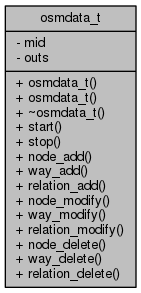
\includegraphics[scale=.85]{input/images/class_osmdata.png}
\caption{Class Diagram of osmdata}
\label{fig:classAnnotation__coll__graph}
\end{figure}
\fi

\begin{figure}
\centering
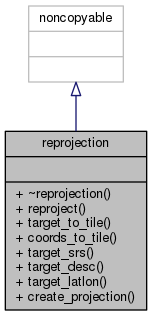
\includegraphics[scale=.85]{input/images/class_reprojection.png}
\caption{Class Diagram for reprojection}
\label{fig:classAnnotation__coll__graphh}
\end{figure}
